\chapter{Introduction}

Unmanned aerial vehicles are airships equipped with embedded systems, sensors and actuators that allow the performance of autonomous or remote controlled flights. They are commonly classified in two groups: rotary-wing vehicles, such as helicopters and quadcopters, and fixed-wing vehicles, such as airplanes.

There is a wide range of applications for UAVs, such as:

\begin{itemize}
	\itemsep0em
	\item Crop dusting;
	\item Herd conduction;
	\item Road monitoring;
	\item Power lines inspection;
	\item Supply deliver in difficult access locations.
\end{itemize}

The simulator presented in this guide is associeted to ProVANT\footnote{provant.paginas.ufsc.br}. ProVANT consists of a partnership between Federal University of Santa Catarina (UFSC) and Federal University of Minas Gearis (UFMG), aiming towards research and development of new technologies to improve the performance of UAVs. In this context, ProVANT currently focuses in the development of tilt-rotor UAVs. The tilt-rotor is an airship with hybrid configuration, featuring the main advantages of both fixed-wing and rotary-wing airships, such as lower power consuption during cruise flights and vertical take-off and landing (VTOL). It can operate both indoors and outdoors.

Currently, ProVANT has three design branches:
\begin{enumerate}
	\item Mechanics/Aerodynamics;
	\item Instrumentation/Electronics;
	\item Control strategy design and state estimation.
\end{enumerate}

The Mechanic/Aerodynamic design alredy has five UAV versions, which were named ProVANT UAV 1.0, 2.0, 2.1, 3.0 and 4.0, shown in Figures \ref{vant1}, \ref{vant2}, \ref{vant21}, \ref{vant3} and \ref{vant4}, respectively. Instrumentation/Electronics is in an advanced stage, having all it's circuits already developed, and improvements are being made on them. As for the Control strategy design and state estimation, several control strategy were developed in the context of this project by master's and doctorate students.

Furthermore, some scientific works were developed. In \cite{Donadel2015}, controllers based on the Linear Quadratic Regulator (LQR), linear $\mathcal{H}_\infty$  and linear mixed $\mathcal{H}_2/\mathcal{H}_\infty$ techniques were developed for ProVANT UAV 1.0, aiming towards path tracking. Some of these controllers were validated by experimental flights. In \cite{Marcelinol2014}, a non-linear control technique based in feedback linearization is presented, dedicated to load transportation in ProVANT UAV 2.0. With the same objective, \cite{Richard2016} presentes the development of a controller based in the Model Predictive Control (MPC) technique. In \cite{Brenner2016}, load transportation in ProVANT UAV 2.0 was addressed, although the path tracking problem was approached from the load's poit of view, to which robust state estimators were developed. In \cite{Daniel2016}, an adaptative control strategy was developed aiming towards path tracking for ProVANT UAV 3.0.

\begin{figure} [H]
	\centering
	\begin{minipage}{.5\textwidth}
		\centering
		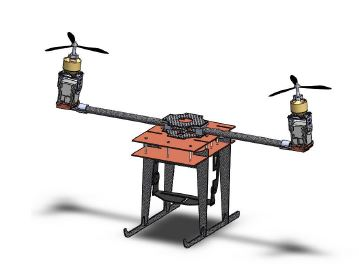
\includegraphics[height=3.5cm]{figuras/VANT1}
		\caption{ProVANT UAV 1.0's mechanical design.}
		\label{vant1}
	\end{minipage}%
	\begin{minipage}{.5\textwidth}
		\centering
		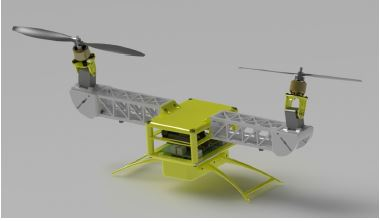
\includegraphics[height=3.5cm]{figuras/VANT2}
		\caption{ProVANT UAV 2.0's mechanical design..}
		\label{vant2}
		\end{minipage}
\end{figure}
				
\begin{figure} [H]
	\centering
	\begin{minipage}{.5\textwidth}
		\centering
		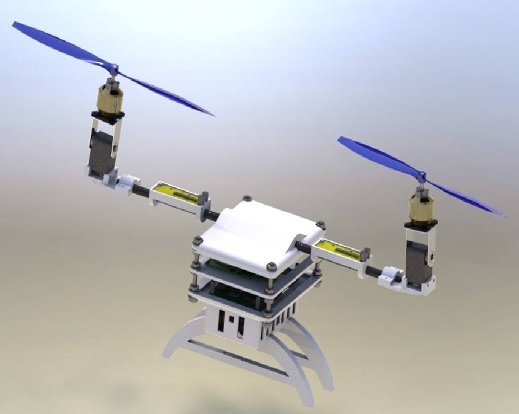
\includegraphics[height=3.5cm]{figuras/VANT21}
		\caption{ProVANT UAV 2.1's mechanical design..}
		\label{vant21}
	\end{minipage}%
	\begin{minipage}{.5\textwidth}
		\centering
		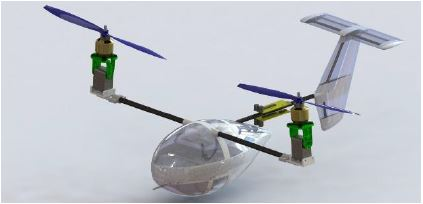
\includegraphics[height=3.5cm]{figuras/VANT3}
		\caption{ProVANT UAV 3.0's mechanical design.}
		\label{vant3}
	\end{minipage}
\end{figure}
							
\begin{figure} [H]
	\centering
	\begin{minipage}{.5\textwidth}
		\centering
		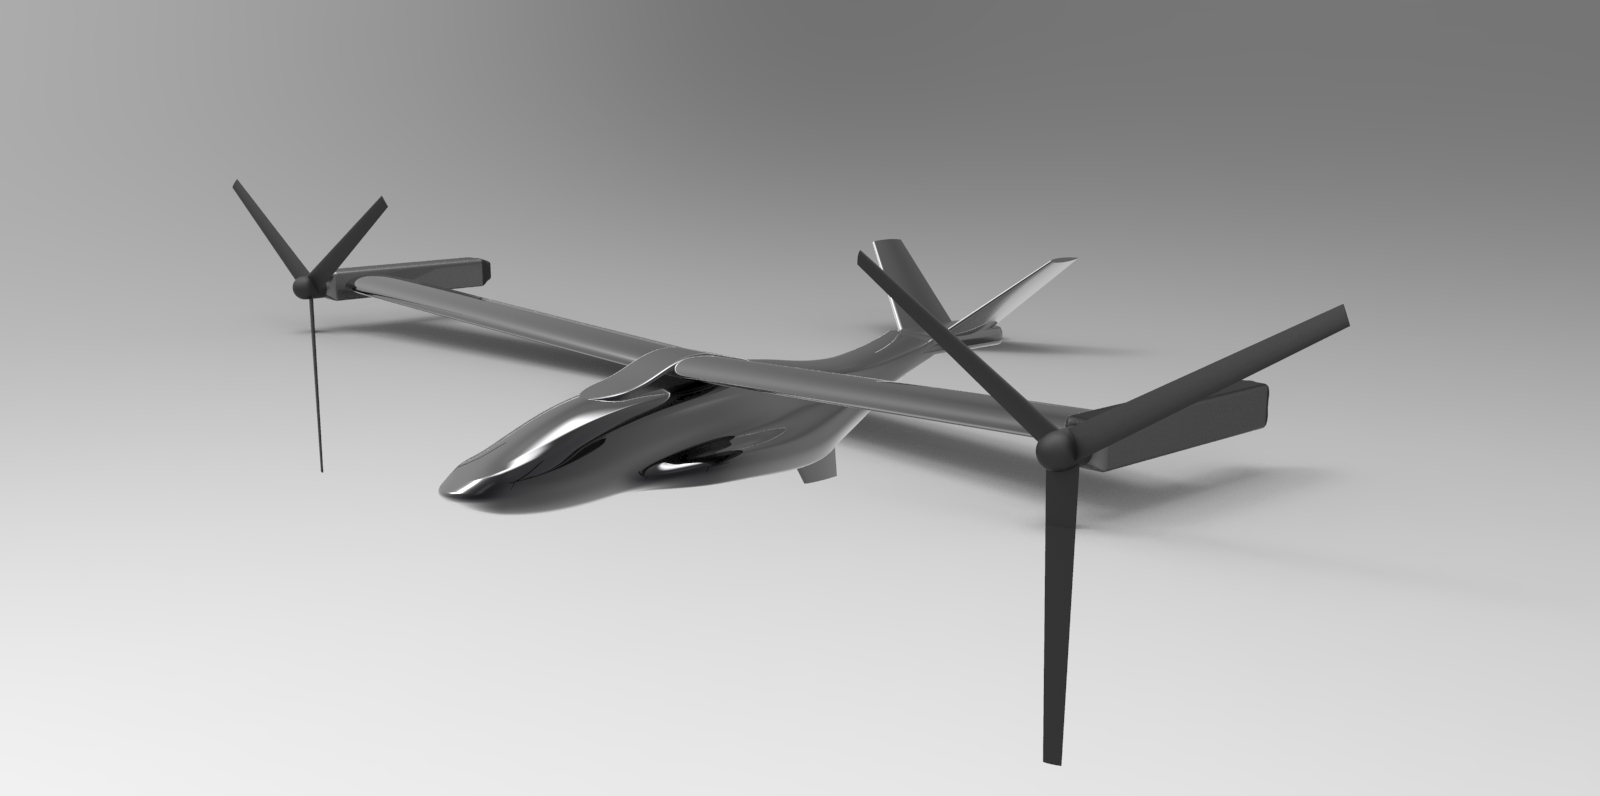
\includegraphics[height=3.5cm]{figuras/VANT4}
		\caption{ProVANT UAV 4.0's mechanical design.}
		\label{vant4}
	\end{minipage}
\end{figure}

ProVANT Simulator was made to be a reliable and easy to use tool, allowing for the reduction of costs and time required for the design and validation of control strategies.